% !TEX encoding = UTF-8 Unicode
\documentclass[10pt, oneside]{book}
% * The documentclass book is a good choice for thesis. For
%   a short text like a course homework the documentclass
%   article would be more suitable.
% * The fontsize specified here is the base text font size 
%   for the document. Headings, footnotes, and other text
%   are automatically scaled relative to that. Typically the
%   documentclass sets a maximum.
% * The option oneside avoids empty pages in drafts, but 
%   should be removed in production: Readers expect chapters
%   to start at the right side. / ... => Do NOT forget
%   to turn on the options inner/outer for geometry after
%   removing oneside!
% 

% check if the editor's file encoding is set accordingly:
\usepackage[utf8]{inputenc}
\usepackage[T1]{fontenc}

% * All languages here are available, but the one named last
%   will be loaded as default for this document.
% * So if you want to use another of these languages as default,
%   you have to switch the order. As a result headers et cetera 
%   will change.
% * ngerman is German with new spelling.
\usepackage[french,ngerman,english]{babel}

% Classic LaTeX would use the \hyphenation{} command.
% Since babel 3.9a* hyphenation can be specified 
% language specific.
% * = introduced 2017, but might require an update
%     depending on your distribution
\babelhyphenation[english]{}
\babelhyphenation[ngerman]{}

% Change left/right to inner/outer once you turn of
% the oneside option!
\usepackage[a4paper,
left = 2.5cm,
right = 6cm, % more space for handwritten notes
top=2.5cm,
bottom=2.5cm]{geometry}

% Load Options for line spacing. The change in 
% spacing is activated later in the document itself.
% For example with \onehalfspacing.
\usepackage{setspace}

% Select a font:
% * That should be a serif type as it is a long text 
%   and serif is better to read than non-serif.
%\usepackage{lmodern}
\usepackage{palatino}



\usepackage{fancyhdr}


% MATH
% * You always need amsmath and amssymb.
\usepackage{amsmath}
\usepackage{amssymb}
\usepackage{cancel} % allows to strike out terms
\usepackage{mathtools}

% TABLES
\usepackage{booktabs} % better looking tables
\usepackage{longtable} % multi-page tables
\usepackage{multirow} % join rows
\usepackage{array}
\usepackage{dcolumn} % align column on a delimiter
\usepackage{tabularx}

% GRAPHICS
\usepackage{graphicx} % Provides \includegraphics{}
\usepackage{tikz}

\usepackage{microtype}


% Format the caption 
\usepackage[
labelfont=bf,
format=hang,
labelsep=colon,
justification=justified,
position=bottom,
figurename=Fig.,
tablename=Tab.]{caption}



% The ulem package makes it possible to underline 
% or strike out text. The option `normalem' avoids 
% redefinition of \emph{}.
\usepackage[normalem]{ulem}

% csquotes introduces the \enquote{} command, which
% sets quotation marks matching the current language.
\usepackage[autostyle=true]{csquotes}

% Changing the footnote style:
\usepackage[marginal]{footmisc}


\usepackage{float}


% Used in this template to generate sample texts.
\usepackage{blindtext}


\usepackage[backend = biber, % because we use utf8 encoding
style=authoryear, % cite with last name author(s) and year
sorting = nyt % how to sort the bibliography
]{biblatex}
\addbibresource{example-literature.bib}


% INDEX
\usepackage{makeidx}
\makeindex

% To show index entries on the page margin use the 
% showidx package. In a draft this is helpful, but 
% before release the package should be removed.
\usepackage{showidx}


% In case we want to show computer code, listings can
% format code in multiple languages.
\usepackage{listings}


% * Hyperrefs allows internal and external links.
% * Once loaded all entries in the table of contents,
%   footnotes, references, ... become hyperlinks in PDF. 
% * Also it has many options to set parameters of 
%   a PDF file.
% * Most of the time it has to be the last package
%   loaded in the preamble.
\usepackage{hyperref}
\hypersetup{
colorlinks = false, 
hidelinks = true, % no boxes around links
bookmarksopen = true,
pdftitle = 'Thesis Example',
pdfauthor = 'Rüdiger Voigt', 
pdfsubject = 'doctoral thesis'}


% The command \today is changed to the current date 
% every time the document gets recompiled.
% A good way to keep track of the version.
\title{A Thesis Template written in \LaTeX}
\author{\foreignlanguage{ngerman}{Rüdiger Voigt, M.A.}}
\date{DRAFT VERSION \today}

\begin{document}


% !TEX encoding = UTF-8 Unicode
% 
% The titlepage-environment is special. It shows no page
% number and the counter is set in a way, that the next 
% page starts as 1.
\begin{titlepage}
% Normally \meaketitle inserts a pagebreak after the title.
% This makes sense, but in the draft phase I want avoid that.
% So instead of just witing \maketitle, I suppress that behavior
% by using the following line:
{\let\newpage\relax\maketitle}
\ \\
\vfill % fill vertical space and push the paragraph below 
% down the page
%
\ \\
% who wrote this thesis? ...
\foreignlanguage{ngerman}{Rüdiger Voigt, M.A.}\\
Student-ID\\
Address\\
Mail / Phone\\
\url{https://www.ruediger-voigt.eu/}\\
\ \\
% Who is the advisor? ...
Advisor: \foreignlanguage{ngerman}{Professor Dr. X}\\
Chair of \dots\\
University of Cologne\\
\end{titlepage}

% include instead of input inserts a pagebreak.
\thispagestyle{empty}
\begin{center}
{\Large Statement}
\end{center}
\ \\
Some universities / departments require a written statement, that everything is the student's own work. For the exact wording consult the corresponding statutes. There might even be rules for the exact place in the document.\\
\ \\
\today in Place\hfill Signature and Name\\
\frontmatter
\tableofcontents
\listoffigures
\listoftables

% \mainmatter switches to arabic numbers for pages.
% It also restart the page counter so content starts
% at page 1.
\mainmatter
% change linespacing via the linespace package:
\onehalfspacing 
% contents divided into multiple files
% !TEX root = thesis.tex\section{Citations}
% !TEX encoding = UTF-8 Unicode

\chapter{Introduction}\label{chapterIntroduction}

\section{Citation Examples}

\cite[635-637]{Beck1995}

\cite[430]{Putnam1988}

Fullcite-Command:

\fullcite{Putnam1988}


\section{Adding Index Entries}

Using the \verb|makeidx| package, you can add entries to the index with \verb|\index{word}| command.
Do not forget the \verb|\makeindex| command in the preamble and run \verb|makeindex| on the document.

Here the index entries are shown in the right margin as the \verb|showidx| is loaded for debugging.

The introduction\index{introduction} is important to stir up reader's curiosity\index{curiosity} and to explain why this is an important topic.\\


\section{Itemize}

\begin{itemize}
	\item first item
	\item second item
	\item third item
\end{itemize}
% !TEX root = thesis.tex
\chapter{Analysis}\label{chapterAnalysis}


\begin{figure}
\centering
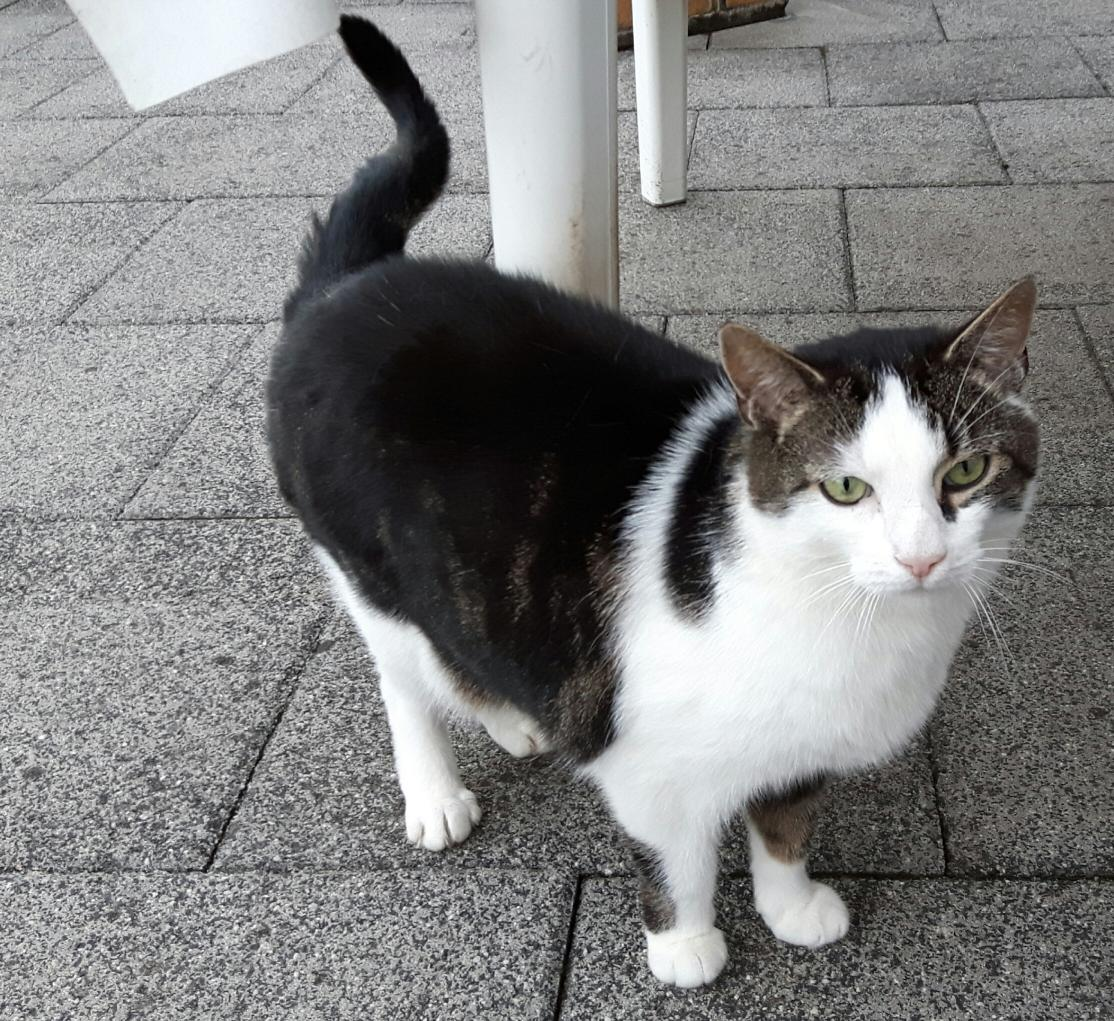
\includegraphics{img/Dala}
\label{img:cat}
\caption{My cat in 2018}
\end{figure}


\begin{figure}
\centering
% Scale the image so it takes up 50% of the width of the text body.
% Height is scaled accordingly.
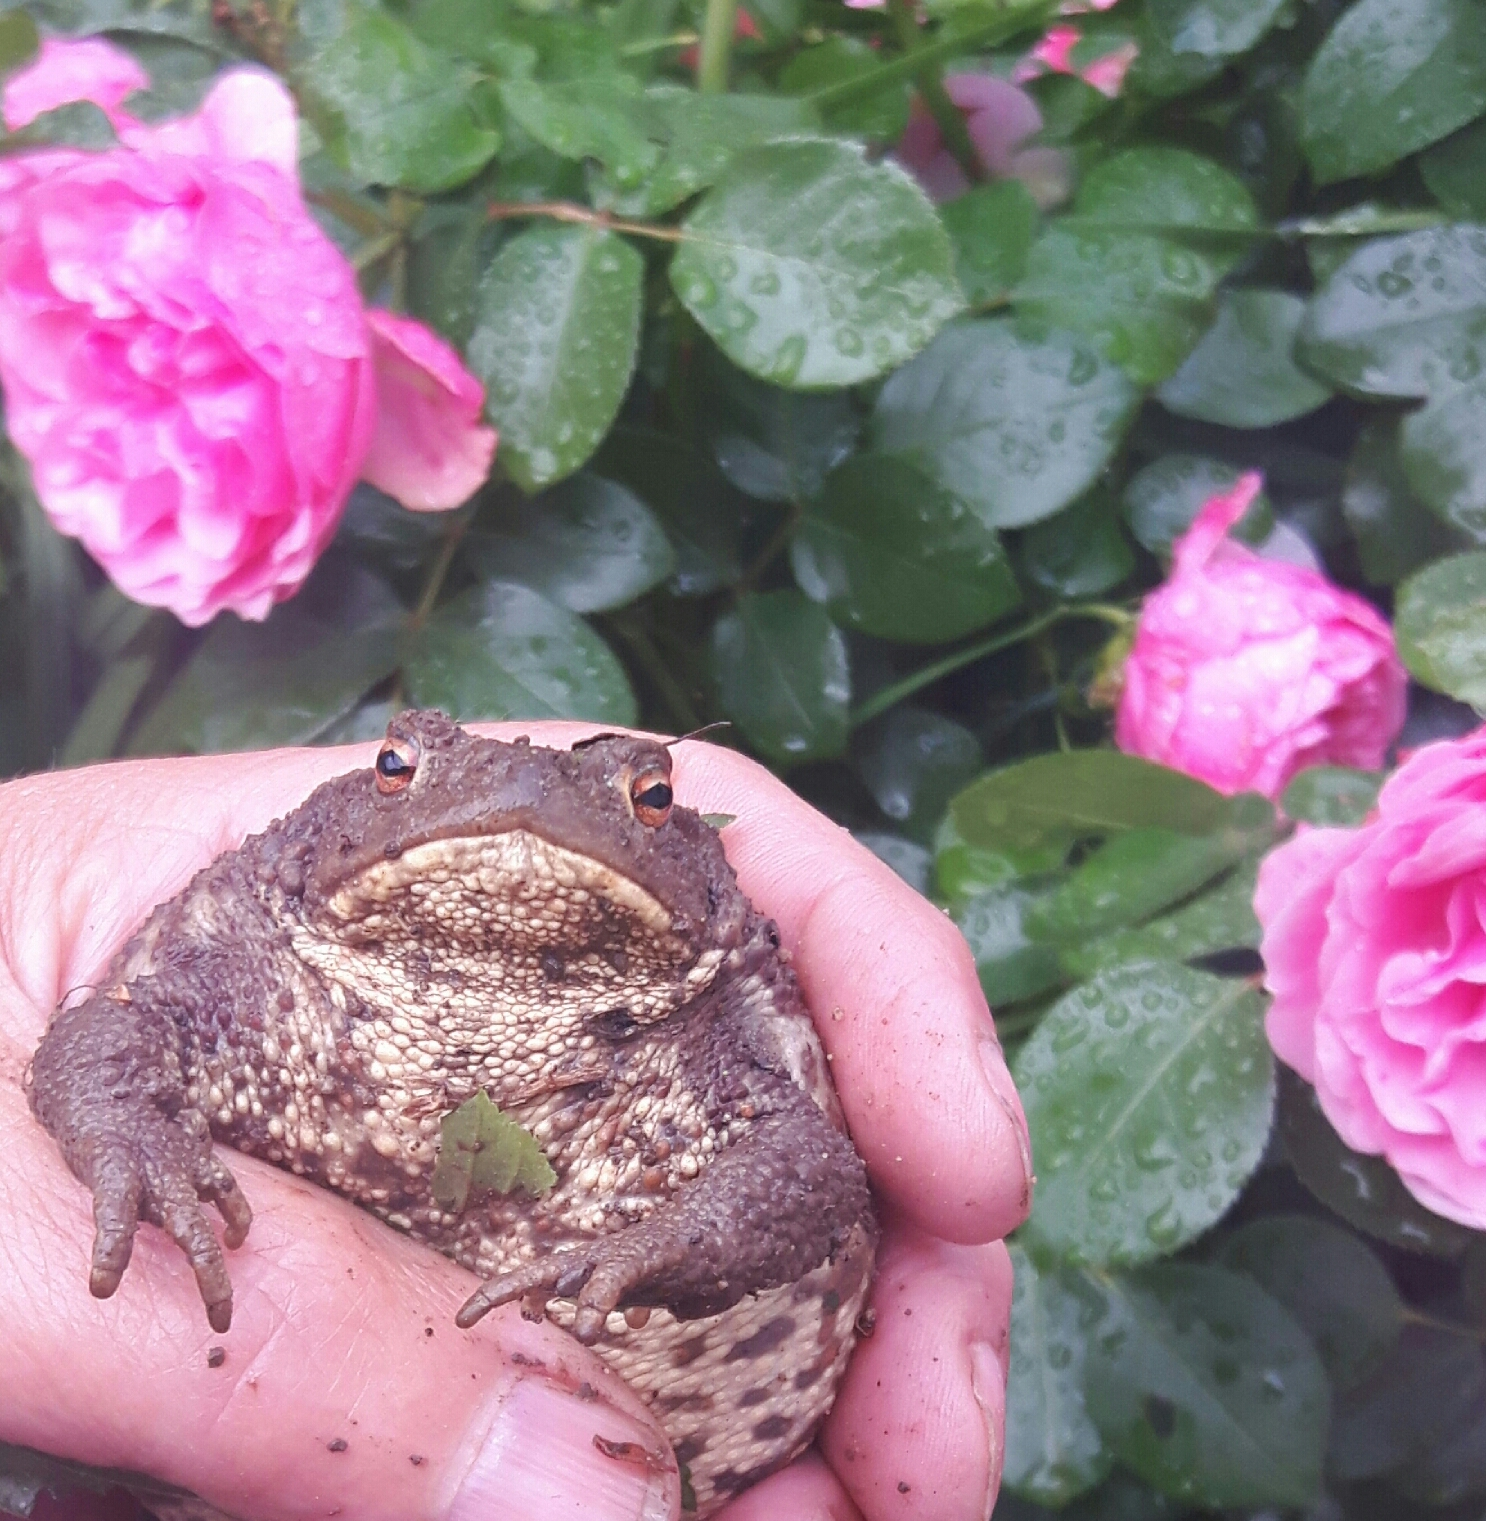
\includegraphics[width=0.5\textwidth]{img/toad}
\label{img:toad}
\caption{A toad found in the garden.}
\end{figure}

% !TEX root = thesis.tex
\chapter{Conclusion}\label{chapterConclusion}

\Blindtext

\appendix
% Chapters (...) get letters instead of numbers.
\chapter{Proof of the Main Result}

\backmatter
\printindex
\printbibliography

\end{document}
